% !TEX root = 0_main.tex
\chapter{Garbled Circuit Synthesis}\label{chap:syn}
In this chapter, first, we review the background of the logic synthesis for digital circuits.
Next, we explain \acrfull{gc} synthesis flow that generates optimized combinational circuits for the \acrshort{gc} protocol using logic synthesis.
Then, we discuss the limitation of logic synthesis techniques and tools for making large combinational circuits for \acrshort{gc}.
A version of this chapter has been published in 2015 IEEE Symposium on Security and Privacy (S\&P) \cite{songhori2015tinygarble}.

\section{Background on Logic Synthesis}\label{sec:syn-back}
Logic synthesis refers to the process of translating an abstract form of function (circuit) presentation to the gate-level logic implementation using a series of sophisticated optimizations, transformations, and mapping \cite{sentovich1992sis,micheli1994synthesis,devadas1994logic,brayton1987mis}.
A logic synthesis tool is a computer program which typically accepts the input circuit in some algorithmic form, logic equation, or even a table, and outputs an implementation suitable for the target hardware platform.
Classic commercial/open-source logic synthesis tools accept the input functions in the \acrfull{hdl} format, e.g., \gls{verilog} or \gls{vhdl} \cite{tool:DesignCompiler,tool:ABC,tool:Encounter,tool:HDLdesigner,tool:PandA,decaluwe2004myhdl} but newer ones also accept high-level format, e.g., \gls{c}/C++ \cite{Gupta2004, tool:Vivado}.
The common target hardware platforms for the synthesized logic include \acrfull{fpga}, \acrfull{pal}, and \acrfull{asic}.

Typical practical implementations of a Boolean function utilize a multi-level network of logic elements.
The tools translate the input to the implementation in two steps: (i) Logic minimization; and (ii) logic optimization.
Logic minimization simplifies the function by combining the separate terms into larger ones containing fewer variables.
The best-known algorithm for logic minimization is the ESPRESSO algorithm \cite{brayton1984logic}; although the resulting minimization is not guaranteed to be the global minimum, it provides a very close approximation of the optimal, while the solution is always free from redundancy.
This algorithm has been incorporated as a standard Boolean function minimization step in virtually any contemporary logic synthesis tool.

Logic optimization takes this minimized format, further processes it, and eventually maps it onto the available basic logic cells or library elements in the target technology (e.g., Lookup tables in \acrshort{fpga} and basic Boolean gates in \acrshort{asic}).

Mapping is limited by factors such as the available gates (logic functions or standard cells) in the technology library, as well as the drive sizes, delay, power, and area characteristics of each gate.

Newer generations of synthesis programs, referred to as \acrfull{hls} tools, accept other forms of input in a higher level programming language \cite{Chapter:Zhang2008,chu1989hyper,corazao1996performance}, e.g., \acrshort{ansi} \gls{c}, C++, SystemC, or Python.
\acrshort{hls} tools are also available in both open-source and commercial forms, e.g., \cite{tool:Vivado,decaluwe2004myhdl,tool:PandA}.
The limitation of the higher level languages is that the behavior of the function is typically decoupled from the timing.
The \acrshort{hls} tools handle the micro-architecture and transform the untimed or partially timed functional code into a fully timed \acrshort{hdl} implementation, which in turn can be compiled by a conventional synthesis tool.
It is well-known that the performance of the circuits resulting from automatically compiled \acrshort{hls} code into \acrshort{hdl} is inferior to the performance of functions directly written in \acrshort{hdl}.
Therefore, the primary driver for the development of \acrshort{hls} tools is user-friendliness and not performance.

\section{TinyGarble GC Synthesis}\label{sec:syn-tiny}
As explained in \sect{ssec:prelim-gc}, Yao's \acrshort{gc} protocol requires a Boolean circuit representation of the underlying function.
Previous work like FairPlay \cite{malkhi2004fairplay} and WYSTERIA \cite{rastogi2014wysteria} used custom-made languages to describe a function and generate the circuit for \acrshort{gc} computation.
In the \gls{tinygarble} framework, the user can write the function in a standard \acrshort{hdl} like \gls{verilog} or \gls{vhdl}.
(She may also write the function in a high-level language like \gls{c} and convert it to \acrshort{hdl} using an \acrshort{hls} tool.)
\gls{tinygarble} uses existing logic synthesis tools to map an \acrshort{hdl} to a list of basic binary gates.
In digital circuit theory, this list is called a \emph{\gls{netlist}}.
The \gls{netlist} is generated based on various constraints and objectives such that it is functionally equivalent to the \acrshort{hdl}/\acrshort{hls} input function.
Exploiting synthesis tools helps to reduce the number of non-XOR gates in the circuit and as a result the total garbling time and communication while also making the framework easily accessible.
In \appx{chap:library}, we provide a library of optimized circuits for complex mathematical/logical operations made by our \acrshort{gc} synthesis approach.

\section{Synthesis Flow}\label{sec:syn-flow}
\fig{fig:synthesis-flow} shows the global flow of \gls{tinygarble} \acrshort{gc} synthesis.
It consists of the following four steps:

\begin{figure}
\centering
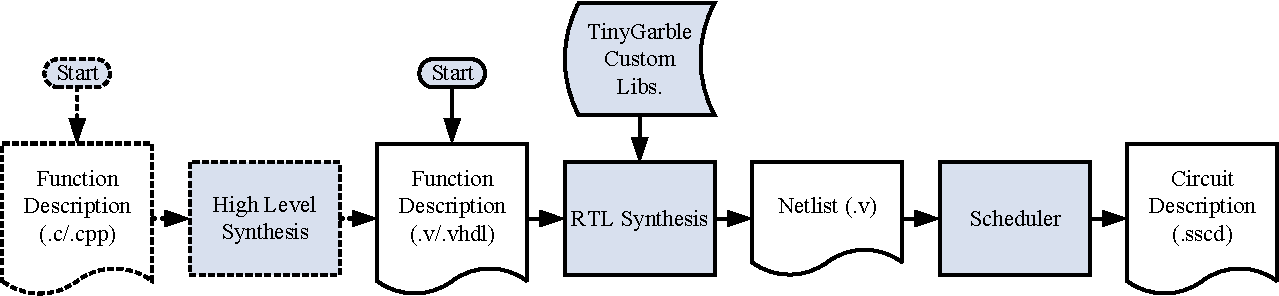
\includegraphics[width=0.95\textwidth]{synthesis_flow-crop.pdf}
\caption{\gls{tinygarble} \acrshort{gc} synthesis flow.
  The inputs can be either a \gls{c}/C++ program (translatable to \acrshort{hdl} via a standard \acrshort{hls} tool) or a direct \acrshort{hdl} description.
  The output is a scheduled circuit description ready to be garbled/evaluated.}
\label{fig:synthesis-flow}
\end{figure}

\begin{enumerate}
\item The input to \gls{tinygarble} \acrshort{gc} synthesis is a file that describes a function written in an \acrshort{hdl} like \gls{verilog} or \gls{vhdl}.
      The function can also be written in a high-level language like \gls{c}/C++ and automatically translated to \acrshort{hdl} using an \acrshort{hls} tool.

\item A standard logic synthesis tool compiles the \acrshort{hdl} to generate the \gls{netlist} file.
      The synthesis tool optimizes the \gls{netlist} based on the user defined objectives/constraints and customized library.
      We set the constraints and library such that the logic synthesis tool produces a \gls{netlist} optimized for evaluation in the \acrshort{gc} protocol.

\item The \gls{netlist} is parsed and topologically sorted.
      Then, we store the sorted \gls{netlist} in a format readable by \gls{tinygarble} \acrshort{gc} engine.
\end{enumerate}

\begin{figure}
\centering
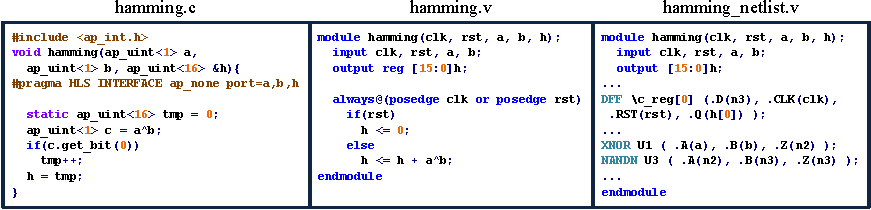
\includegraphics[width=\textwidth]{HLS_HDL_netlist-crop.pdf}
\caption{Sample files at the different steps of \gls{tinygarble} \acrshort{gc} synthesis flow for Hamming distance function.}
\label{fig:globalflow_sample}
\end{figure}

\fig{fig:globalflow_sample} shows examples of files at different steps of \gls{tinygarble} \acrshort{gc} synthesis flow for Hamming distance function.
The \textsl{hamming.c} file contains the description of the function in the \gls{c} language.
The user inputs this function to an \acrshort{hls} tool to generate the corresponding description in \gls{verilog}.
The resulting \gls{verilog} file is functionally similar to the \textsl{hamming.v} file shown in the figure, but it may look more complicated and be less efficient since it is generated by an automated tool.
A user can also write the description directly in \gls{verilog} to have more control of the circuit and therefore a more optimized \gls{netlist}.
We provide the \textsl{hamming.v} file to a logic synthesis tool along with the \gls{tinygarble} custom libraries to generate \gls{netlist} \textsl{hamming\_netlist.v}.
The \gls{netlist} describes the same function as \textsl{hamming.c} and \textsl{hamming.v} but uses the logic cells provided in the technology library.
The technology library contains 2-input-1-output logic cells to be compatible the \acrshort{gc} protocol.

In the following, we describe the details of the synthesis steps and how we manipulate the synthesis tools in each of the steps to generate optimized \gls{netlist}s for the \acrshort{gc} protocol.

\section{Synthesis Library}\label{sec:syn-synlib}
The first phase in the synthesis flow is to convert arithmetic and conditional operations like add, multiply, and if-else to their logical representations that fit best to the user's constraints.
For example, we can replace the sum of two N-bit numbers with an N-bit ripple carry adder in the case of area optimization or an N-bit carry look-ahead adder for timing optimization.
A library that consists of these various implementations is called a \emph{synthesis library}.
We develop our synthesis library that includes implementations customized for the \acrshort{gc} protocol.
In this library, we build the arithmetic operations based on a full adder with one non-XOR gate \cite{boyar2006concrete} and conditional operations based on a 2-to-1 \acrfull{mux} with one non-XOR gate \cite{kolesnikov2008improved}.

\section{Technology Library}\label{sec:syn-techlib}
The next step is to map the structural representation onto a \emph{technology library} to generate the \gls{netlist}.
A technology library contains basic units available on the target platform.
For example, tools targeting \acrfull{fpga} like Xilinx ISE or Quartus provide \acrfull{lut} and \acrfull{ff} in their technology libraries, which form the architecture of an \acrshort{fpga}.
On the other hand, tools targeting \acrfull{asic} like \gls{synopsys-dc}, Cadence, and ABC, may contain a more diverse collection of elements starting from basic gates like XOR and AND to more complex units like \acrshort{ff}s.
The technology library includes logical descriptions of these units along with their performance parameters like delay and area.
The goal of the synthesis tool in this step is to generate a \gls{netlist} of library components that best fit the given constraints.
For logic synthesis, we use tools targeting \acrshort{asic}s as they allow more flexibility in their input technology library.
We design a custom technology library that contains two-input gates as they incur minimum garbled tables in the \acrshort{gc} protocol compared to gates with more inputs.
We set the area of XOR gates to 0 and that of non-XOR gates to a non-0 value, e.g., 1.
We choose area minimization as the only optimization goal, so the synthesis tool produces a \gls{netlist} with the minimum possible number of non-XOR gates.
Reducing non-XOR gates translates directly into decreasing the communication cost of the GC protocol due to the Free XOR optimization \cite{kolesnikov2008improved}.

An additional feature of our custom technology library is that it contains non-standard gates (other than basic gates like NOT, AND, NAND, OR, NOR, XOR, and XNOR) to increase the flexibility of mapping process.
For example, the logical functions $F = A\wedge B$ and $F = (\neg A)\wedge B$ requires same effort in garbling/evaluation.
However, using only standard gates, the second function would need two gates (a NOT gate and an AND gate) and store one extra pair of labels for $\neg A$ in the memory.
We include four such non-standard gates with an inverted input in our custom library.
XOR, XNOR, and NOT gates are free, so we set their area to 0.
We assign the area of all other gates, similar to that of non-XOR, to 1.
To be consistent with the previous work in the literature, we use ``number of non-XOR gates'' to refer to the number of non-free gates in a circuit throughout this thesis.
Due to the Free XOR optimization, this metric directly corresponds to time and communication cost of garbling/evaluating the circuit.

\section{Offline Circuit Synthesis}\label{sec:syn-offline}
In \gls{tinygarble} \acrshort{gc} synthesis, we use logic synthesis tools in an offline manner to generate a circuit for a given functionality.
This offline synthesis followed by a topological sort provides a ready-to-use circuit description for any \acrshort{gc} implementations including our \gls{tinygarble} \acrshort{gc} engine.
This approach, unlike online circuit generation, does not require misspending time for producing the circuit during garbling/evaluation.
It also enables employing useful synthesis optimization techniques that were previously infeasible for the online generation.
Moreover, the synthesis tools have a global view of the circuit, unlike previous work that manually optimized small modules of the circuit.
This overall view allows logic synthesis tools to provide more efficient optimization for any arbitrary function and set of constraints.

\section{Limitation}\label{sec:syn-limit}
The synthesis approach has certain limitations when it comes to generating combinational circuits for extremely large functions.
The amount of memory and computation resources required by logic synthesis tools considerably increase for producing large combinational circuits.
Synthesis tools are not designed to support such large scale combinational circuits.
Thus, the \acrshort{gc} synthesis approach cannot scale, at least automatically, for generating combinational circuits for large functions.

However, most of these large functions include one or more recurring computation blocks (a.k.a, loops).
In combinational representation, these loops have to be unfolded and represented as repeated blocks in the circuits.
In hardware design, these functions are folded around their loops and are described using sequential circuits.
A sequential circuit has feedback loops and is evaluated for multiple times (sequential cycles).
Thus, it is the most suited format to represent the recurring blocks in large functions
In the next chapter, we will discuss the possibility of using the sequential circuit for the \acrshort{gc} protocol.
We will show how we can exploit loops in sequential circuits to fold large functions while still benefiting from the optimization of synthesis tools.
